
% Lab 2 Handout

\labtitle{\semester}{Big-Oh}{TBD}

\section*{Learning Goals}
During this lab, you will:
\begin{itemize}
    \item review Bachmann-Landau notation
    \item examine certain functions and their relative asymptotic growth rates
    \item examine the runtime complexity of code
    \item prove Bachmann-Landau relations
\end{itemize}

\section*{Big-Oh and Bachmann-Landau Notation}

In class, you have started to discuss Big Oh and other ways of classifying functions and algorithms. These notations belong to what is commonly referred to as the \textit{Bachmann-Landau} family of notations.
    
\begin{framed}\relax
    \begin{center}\relax
        \underline{Big-Oh Notation}
    \end{center}
    \textbf{Definition.} $f(n) = O(g(n))$ if there exist constants $n_0$ and $c > 0$ s.t. $f(i) \leq c g(i)$ for all $i \geq n_0$.\\

    Simplified: If $f(n)$ is $O(g(n))$, $g(n)$ is an asymptotic upper bound for $f(n)$.
\end{framed}
\begin{figure}[h]
    \centering
    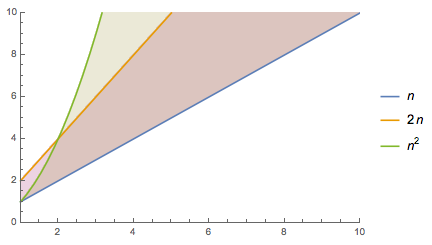
\includegraphics[width=\textwidth*9/16]{big_oh_1}
    \caption*{$n = O(n)$, $n = O(n^2)$}
\end{figure}

\begin{framed}
    \begin{center}
        \underline{Big-Omega Notation}
    \end{center}
    \textbf{Definition.} $f(n) = \Omega(g(n))$ if there exist constants $n_0$ and $c > 0$ s.t. $f(i) \geq c g(i)$ for all $i \geq n_0$.\\

    Simplified: If $f(n)$ is $\Omega(g(n))$, $g(n)$ is an asymptotic lower bound for $f(n)$.
\end{framed}
\begin{figure}[h]
    \centering
    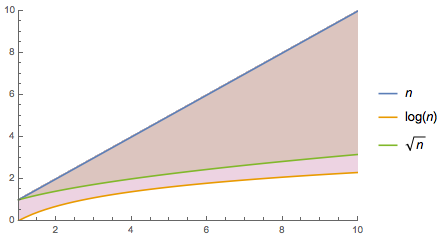
\includegraphics[width=\textwidth*9/16]{big_oh_2}
    \caption*{$n = \Omega(\lg n)$, $n = \Omega(\sqrt{n})$}
\end{figure}

\begin{framed}
    \begin{center}
        \underline{Big-Theta Notation}
    \end{center}
    \textbf{Definition.} $f(n) = \Theta(g(n))$ if $f(n) = O(g(n))$ and $f(n) = \Omega(g(n))$.\\

    Simplified: If $f(n)$ is $\Theta(g(n))$, $g(n)$ is an asymptotic \textit{tight} bound for $f(n)$.
\end{framed}

\begin{figure}[h]
    \centering
    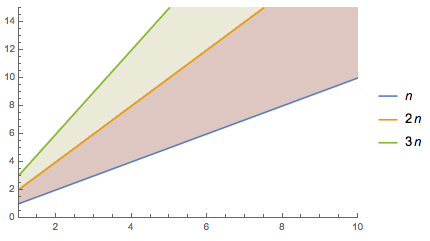
\includegraphics[width=\textwidth*9/16]{big_oh_3}
    \caption*{$n = \Theta(n)$. Every function is Big-$\Theta$ of itself.}
\end{figure}

As a protip, it is also good to note that the Bachmann-Landau notations refer to \textit{classes of functions}. When you read $f(n) = O(g(n))$, this is equivalent to the statement: $$f(n) \in O(g(n))$$. Specifically, $f(n)$ is in the class of functions which are asymptotically bounded above by $g(n)$. Likewise, Big-$\Omega$ and Big-$\Theta$ both reflect classes of functions.

\begin{framed}
    \begin{center}
        \underline{Stirling's Approximation}
    \end{center}
    $$n! \sim (\frac{n}{e})^n \sqrt{2\pi n}$$
\end{framed}

\section*{Lab Problems}

\subsection*{Problem 1}
Order the following functions such that if $f$ precedes $g$, then $f(n)$ is $O(g(n))$.

\begin{center}
    $\sqrt{n}$, $n$, $n^{1.5}$, $n^2$, $n \lg{n}$, $n\lg\lg{n}$, $n\lg{n^2}$, $2^{n/2}$, $2^n$, $\lg(n!)$, $n^2\lg{n}$, $n^3$, $2^{2^n}$
\end{center}

\subsection*{Problem 2}
Provide a runtime analysis of the following loop:

\begin{verbatim}
    for(int i = 0; i < n; i++)
        for (int j = i; j <= n; j++)
            for (int k = i; k <= j; k++)
                sum++;
\end{verbatim}

\subsection*{Problem 3}
In this problem, you are \textbf{not} allowed to use the theorems about Big-Oh stated in the lecture notes. Your proof should follow exclusively from the definition of Big-Oh.\\

Prove or disprove the following statement:
\begin{center}
    $f(n) + g(n)$ is $\Theta(\max\big\{f(n),g(n)\big\}),$ where $f, g:R\rightarrow R^{+}$.
\end{center}

\subsection*{Problem 4}
Prove or disprove the following statement:
\begin{center}
    $2^n$ is $O(n!)$.
\end{center}

\subsection*{Problem 5}
Provide a runtime analysis of the following loop:

\begin{verbatim}
    for (int i = 2; i < n; i = i*i)
        for (int j = 1; j < Math.sqrt(i); j = j+j)
            System.out.println("*");
\end{verbatim}

\subsection*{Problem 6}
Prove or disprove the following statement:

\begin{center}
    $\lg(n!)$ is $\Theta(n\lg{n})$.
\end{center}

\newpage

\section*{Logarithms Cheat Sheet}

Exponential terms appear very frequently in the study of algorithms and their runtimes. Therefore, logarithms are very useful when manipulating exponential terms in Big-Oh proofs! It is therefore advised that you become very familiar with logs.\\

Here's a little cheat-sheet for you to refresh your memory!

\begin{framed}
    \begin{center}
        \underline{Properties of Logarithms}
    \end{center}
    $$\log(c\cdot f(n)) = \log c + \log f(n)$$
    $$\log x^y = y \log x$$
    $$\log a + \log b = \log(ab)$$
    $$\log a - \log b = \log(a/b)$$
    $$\log_b x = \frac{\log_c x}{\log _c b}$$
    $$\log 2^n = n$$
    $$\log n! = \log [n\cdot(n-1)...2 \cdot 1] = \log n + \log(n-1) + ... + \log 1 = \sum_{i = 1}^n \log i$$
\end{framed}
